\subsection{Second Attempt}
\label{sec:setup.quad.hyper.2}

Now, we try to close the gaps between the ``type A'' parameter regions of one sequence of parameter regions with the same period to form proper chains.
For this, we change the parameters of the function $g_L$ and therefore the shape of the branches $f_\A$ and $f_\C$.
We fix $a_L = 4$ and $b_L = -\frac{1}{2}$.
This causes the branches $f_\A$ and $f_\B$ to be more shallow than before with $a_L = 8$ and $b_L = -1$.

All other fixed parameters stay the same as before.
Scanning the periods of the stable cycles in the ranges $\alpha \in [0.275, 0.35]$ and $\beta \in [0.15, 0.1875]$ results in the diagrams in \Cref{fig:setup.quad.hyper.2.period}.
We can see in \Cref{fig:setup.quad.hyper.2.period.full}, that the gap between the ``type A'' parameter regions of a sequence with the same period closed.
Also, there are these parameter regions in the chains, for example at point $C$, where the chains get narrower.
The same thing is observed in the original model and those regions are ``type B'' parameter regions in the original model.

Plotting the same diagram, but with an adjusted model, highlights ``type B'' parameter regions.
The adjusted model is the halved model, it is explained in detail in \Cref{chap:add}.
For now, the only important thing is that ``type B'' parameter regions of a chain have a significantly higher period than the ``type A'' parameter regions of the same chain in this adjusted model.
The result is \Cref{fig:setup.quad.hyper.2.period.halved}.
We can see clearly that ``type A'' and ``type B'' parameter regions alternate in the chains, just as in the original model.

\begin{figure}
	\centering
	\begin{subfigure}{0.4\textwidth}
		\centering
		\includegraphics[width=\textwidth]{41_Quadratic_fittingR_Gecko/2D_Period_Whole/result.png}
		\caption{Full Model}
		\label{fig:setup.quad.hyper.2.period.full}
	\end{subfigure}
	\begin{subfigure}{0.4\textwidth}
		\centering
		\includegraphics[width=\textwidth]{42_Quadratic_fittingR_Gecko_Halved/2D_Period_Whole/result.png}
		\caption{Halved Model}
		\label{fig:setup.quad.hyper.2.period.halved}
	\end{subfigure}
	\caption[2D scan of the periods of the quadratic model with hyperparameters for different values of the fixed parameters]{
	2D scan of the periods of the piecewise quadratic model with hyperparameters $g_R\left(\frac{1}{4}\right), g_R\left(\frac{1}{2}\right),$ and $\left. \frac{d}{dx} g_R\left(x\right) \right|_{x = \frac{1}{2}}$.
	The parameters $a_L = 4, b_L = -\frac{1}{2}, g_R\left(\frac{1}{4}\right) = 0.525,$ and $\left. \frac{d}{dx} g_R\left(x\right) \right|_{x = \frac{1}{2}} = 1.2$ are fixed.
	The parameters $\alpha = g_R\left(\frac{1}{4}\right)$ and $\beta = c_L$ are varied in the ranges $[0.275, 0.35]$ and $[0.15, 0.1875]$, respectively.
	The points $A, B,$ and $C$ mark the parameter values used for the cobweb diagrams in \Cref{fig:setup.quad.hyper.2.cobwebs}.
	(a) shows the scan for the normal model as defined above, while (b) shows the scan for the adjusted model where we can see ``type B'' parameter regions as they have higher periods in the adjusted model.
	}
	\label{fig:setup.quad.hyper.2.period}
\end{figure}

\begin{figure}
	\centering
	\begin{subfigure}{0.3\textwidth}
		\centering
		\includegraphics[width=\textwidth]{41_Quadratic_fittingR_Gecko/Cobweb_A/result.png}
		\caption{At Point $A$}
		\label{fig:setup.quad.hyper.2.cobweb.A}
	\end{subfigure}
	\begin{subfigure}{0.3\textwidth}
		\centering
		\includegraphics[width=\textwidth]{41_Quadratic_fittingR_Gecko/Cobweb_B/Manual/result.png}
		\caption{At Point $B$}
		\label{fig:setup.quad.hyper.2.cobweb.B}
	\end{subfigure}
	\begin{subfigure}{0.3\textwidth}
		\centering
		\includegraphics[width=\textwidth]{41_Quadratic_fittingR_Gecko/Cobweb_C/result.png}
		\caption{At Point $C$}
		\label{fig:setup.quad.hyper.2.cobweb.C}
	\end{subfigure}
	\caption[Cobwebs of the piecewise quadratic model with hyperparameters for different values of the fixed parameters]{
	Cobweb diagrams at three parameter values of $\alpha = g_R\left(\frac{1}{4}\right)$ and $\beta = c_L$ in the piecewise quadratic model with hyperparameters.
	The other parameters are fixed as $a_L = 4, b_L = -\frac{1}{2}, g_R\left(\frac{1}{2}\right) = \frac{1}{2} + \frac{1}{40}$, and $\left. \frac{d}{dx} g_R(x) \right|_{x = \frac{1}{2}} = 1 + \frac{1}{5}$.
	The parameter values are marked in \Cref{fig:setup.quad.hyper.2.period}.
	(a) shows the cycle $\Cycle{\A^7\B^8\C^7\D^8}$ at point $A$, (b) shows the two coexisting cycles $\Cycle{\A^7\B^8\C^7\D^8}$ (green) and $\Cycle{\A^6\B^9\C^6\D^9}$ (red) at point $B$, and (c) shows the cycle $\Cycle{\A^6\B^9\C^6\D^9}$ at point $C$.
	}
	\label{fig:setup.quad.hyper.2.cobwebs}
\end{figure}

We also check the cobweb diagrams of the stable cycles along a chain.
\Cref{fig:setup.quad.hyper.2.cobwebs} contains the cobwebs for all marked points in \Cref{fig:setup.quad.hyper.2.period}.
All cycles of this chain have period $30$.
The symbolic sequence of the cycle at point $A$ is $\A^7\B^8\C^7\D^8$.
It is a symmetric cycle and therefore the parameter regions is of ``type A''.
The symbolic sequence of the cycle at point $C$ is $\A^6\B^9\C^6\D^9$.
It is also a symmetric cycle and this parameter regions is also of ``type A''.
It is the next ``type A'' parameter region in the chain after the parameter regions of point $A$.
And just like in the original model, one point of each of the branches $f_\A$ and $f_\C$ moved to the branch $f_\B$ and $f_\D$, respectively.

Between those two ``type A'' parameter regions there is a narrower parameter region with the same period.
It is marked with point $C$.
At this point, there are 2 coexisting cylces of period 30.
Their symbolic sequences are $\A^7\B^8\C^6\D^9$ and $\A^6\B^9\C^7\D^8$, respectively.
This is exactly the same behavior, that the original model shows.
Between two ``type A'' parameter regions there is a ``type B'' parameter region where the cycles behave like either cycle of the ``type A'' parameter regions before and after this ``type B'' parameter region on each half of the model.
